% Processing pipeline. Compile standalone:
%   pdflatex -output-directory=generated figures/pipeline.tex
\documentclass[border=4pt]{standalone}
\usepackage{tikz}
\usetikzlibrary{arrows.meta, positioning, shapes.geometric}

\begin{document}
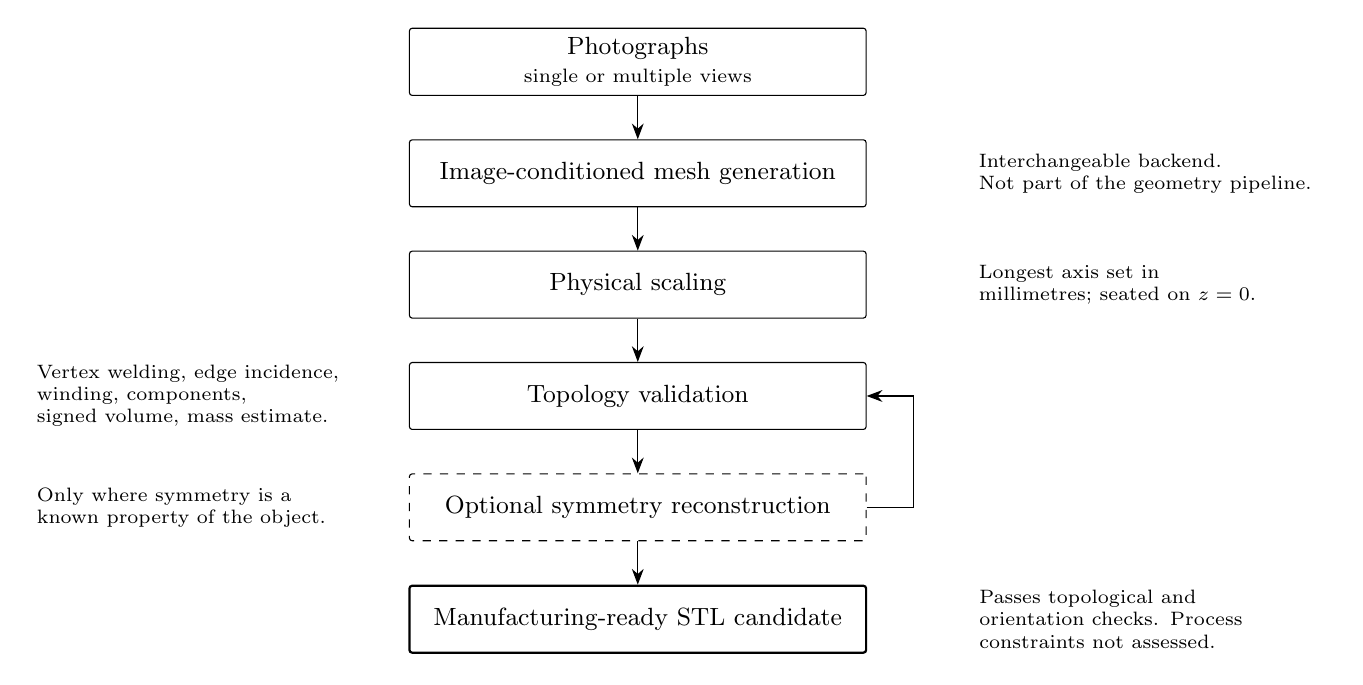
\begin{tikzpicture}[
  node distance = 5.5mm,
  every node/.style = {font=\small},
  stage/.style = {
    draw, rectangle, rounded corners=1pt, line width=0.4pt,
    minimum width=58mm, minimum height=8.5mm, align=center
  },
  optional/.style = {stage, dashed},
  terminal/.style = {stage, line width=0.8pt},
  note/.style = {font=\scriptsize, align=left, text width=44mm},
  flow/.style = {-{Stealth[length=2mm]}, line width=0.4pt}
]

\node[stage] (input) {Photographs \\[-1pt] \scriptsize single or multiple views};
\node[stage, below=of input] (generate) {Image-conditioned mesh generation};
\node[stage, below=of generate] (scale) {Physical scaling};
\node[stage, below=of scale] (validate) {Topology validation};
\node[optional, below=of validate] (symmetry) {Optional symmetry reconstruction};
\node[terminal, below=of symmetry] (output) {Manufacturing-ready STL candidate};

\draw[flow] (input) -- (generate);
\draw[flow] (generate) -- (scale);
\draw[flow] (scale) -- (validate);
\draw[flow] (validate) -- (symmetry);
\draw[flow] (symmetry) -- (output);

% Revalidation after the optional symmetry pass.
\draw[flow] (symmetry.east) -- ++(6mm,0) |- (validate.east);

\node[note, right=13mm of generate.east, anchor=west]
  {Interchangeable backend. \\ Not part of the geometry pipeline.};
\node[note, right=13mm of scale.east, anchor=west]
  {Longest axis set in \\ millimetres; seated on $z=0$.};
\node[note, right=13mm of output.east, anchor=west]
  {Passes topological and \\ orientation checks. Process \\ constraints not assessed.};

\node[note, left=6mm of validate.west, anchor=east, text width=40mm]
  {Vertex welding, edge incidence, \\ winding, components, \\ signed volume, mass estimate.};
\node[note, left=6mm of symmetry.west, anchor=east, text width=40mm]
  {Only where symmetry is a \\ known property of the object.};

\end{tikzpicture}
\end{document}
